\documentclass[11pt]{article}

\usepackage[colorlinks=true]{hyperref}

% This is a toggle for whether the solutions should be included in output of this document
\newif\ifSolutions
%\Solutionsfalse  % this is used to exclude the solutions
\Solutionstrue  % this is used to include the solutions


\usepackage[left=0.8in, right=0.8in, top=0.7in, bottom=1in, includefoot]{geometry}
\usepackage{fancyhdr}
\usepackage{array}
\usepackage{multicol}
\setlength{\parindent}{0mm}
\setlength{\parskip}{5pt}
\usepackage{sectsty}
\allsectionsfont{\sffamily}
\setlength{\headheight}{2cm}
\usepackage{amsmath,amssymb,bm}
\usepackage{booktabs}
\usepackage{graphicx}
\usepackage{color}
\usepackage{cancel}
\usepackage{comment}
\usepackage{hyperref}
\usepackage{subfig}
\usepackage{multirow}
\usepackage{placeins}

% Global definitions
%
% boldface letters
%
%\newcommand{\boldface}[1]{\mathbf{#1}}   % upright
\newcommand{\boldface}[1]{\boldsymbol{#1}}  % italic (slanted)
%
\newcommand{\bfa}{\boldface{a}}
\newcommand{\bfb}{\boldface{b}}
\newcommand{\bfc}{\boldface{c}}
\newcommand{\bfd}{\boldface{d}}
\newcommand{\bfe}{\boldface{e}}
\newcommand{\bff}{\boldface{f}}
\newcommand{\bfg}{\boldface{g}}
\newcommand{\bfh}{\boldface{h}}
\newcommand{\bfi}{\boldface{i}}
\newcommand{\bfj}{\boldface{j}}
\newcommand{\bfk}{\boldface{k}}
\newcommand{\bfl}{\boldface{l}}
\newcommand{\bfm}{\boldface{m}}
\newcommand{\bfn}{\boldface{n}}
\newcommand{\bfo}{\boldface{o}}
\newcommand{\bfp}{\boldface{p}}
\newcommand{\bfq}{\boldface{q}}
\newcommand{\bfr}{\boldface{r}}
\newcommand{\bfs}{\boldface{s}}
\newcommand{\bft}{\boldface{t}}
\newcommand{\bfu}{\boldface{u}}
\newcommand{\bfv}{\boldface{v}}
\newcommand{\bfw}{\boldface{w}}
\newcommand{\bfx}{\boldface{x}}
\newcommand{\bfy}{\boldface{y}}
\newcommand{\bfz}{\boldface{z}}
%
\newcommand{\bfA}{\boldface{A}}
\newcommand{\bfB}{\boldface{B}}
\newcommand{\bfC}{\boldface{C}}
\newcommand{\bfD}{\boldface{D}}
\newcommand{\bfE}{\boldface{E}}
\newcommand{\bfF}{\boldface{F}}
\newcommand{\bfG}{\boldface{G}}
\newcommand{\bfH}{\boldface{H}}
\newcommand{\bfI}{\boldface{I}}
\newcommand{\bfJ}{\boldface{J}}
\newcommand{\bfK}{\boldface{K}}
\newcommand{\bfL}{\boldface{L}}
\newcommand{\bfM}{\boldface{M}}
\newcommand{\bfN}{\boldface{N}}
\newcommand{\bfO}{\boldface{O}}
\newcommand{\bfP}{\boldface{P}}
\newcommand{\bfQ}{\boldface{Q}}
\newcommand{\bfR}{\boldface{R}}
\newcommand{\bfS}{\boldface{S}}
\newcommand{\bfT}{\boldface{T}}
\newcommand{\bfU}{\boldface{U}}
\newcommand{\bfV}{\boldface{V}}
\newcommand{\bfW}{\boldface{W}}
\newcommand{\bfX}{\boldface{X}}
\newcommand{\bfY}{\boldface{Y}}
\newcommand{\bfZ}{\boldface{Z}}

\newcommand{\bfFe}{\boldface{F}_{\text{e}}}
\newcommand{\bfFp}{\boldface{F}_{\text{p}}}
\newcommand{\bfepse}{\pmb{\varepsilon}_{\text{e}}}
\newcommand{\bfepsp}{\pmb{\varepsilon}_{\text{p}}}
\newcommand{\bfeps}{\pmb{\varepsilon}}

%
% boldface greek symbols
%
\newcommand{\bfalpha}{\boldsymbol{\alpha}}
\newcommand{\bfbeta}{\boldsymbol{\beta}}
\newcommand{\bfgamma}{\boldsymbol{\gamma}}
\newcommand{\bfdelta}{\boldsymbol{\delta}}
\newcommand{\bfepsilon}{\pmb{\varepsilon}}
\newcommand{\bfzeta}{\boldsymbol{\zeta}}
\newcommand{\bfeta}{\boldsymbol{\eta}}
\newcommand{\bftheta}{\boldsymbol{\theta}}
\newcommand{\bfkappa}{\boldsymbol{\kappa}}
\newcommand{\bflambda}{\boldsymbol{\lambda}}
\newcommand{\bfrho}{\boldsymbol{\rho}}
\newcommand{\bfmu}{\boldsymbol{\mu}}
\newcommand{\bfnu}{\boldsymbol{\nu}}
\newcommand{\bfpi}{\boldsymbol{\pi}}
\newcommand{\bfxi}{\boldsymbol{\xi}}
\newcommand{\bfsigma}{\boldsymbol{\sigma}}
\newcommand{\bftau}{\boldsymbol{\tau}}
\newcommand{\bfphi}{\boldsymbol{\phi}}
\newcommand{\bfvarphi}{\boldsymbol{\varphi}}
\newcommand{\bfchi}{\boldsymbol{\chi}}
\newcommand{\bfomega}{\boldsymbol{\omega}}
\newcommand{\bfnull}{\boldsymbol{0}}
%
\newcommand{\bfGamma}{\boldsymbol{\Gamma}}
\newcommand{\bfDelta}{\boldsymbol{\Delta}}
\newcommand{\bfTheta}{\boldsymbol{\Theta}}
\newcommand{\bfLambda}{\boldsymbol{\Lambda}}
\newcommand{\bfPi}{\boldsymbol{\Pi}}
\newcommand{\bfXi}{\boldsymbol{\Xi}}
\newcommand{\bfSigma}{\boldsymbol{\Sigma}}
\newcommand{\bfPhi}{\boldsymbol{\Phi}}
\newcommand{\bfChi}{\boldsymbol{\Chi}}
\newcommand{\bfOmega}{\boldsymbol{\Omega}}
\newcommand{\bfnabla}{\boldsymbol{\nabla}}
\newcommand{\laplace}{\boldsymbol{\Delta}}
%
% caligraphic letters
%
\newcommand{\calA}{\mathcal{A}}
\newcommand{\calB}{\mathcal{B}}
\newcommand{\calC}{\mathcal{C}}
\newcommand{\calD}{\mathcal{D}}
\newcommand{\calE}{\mathcal{E}}
\newcommand{\calF}{\mathcal{F}}
\newcommand{\calG}{\mathcal{G}}
\newcommand{\calH}{\mathcal{H}}
\newcommand{\calI}{\mathcal{I}}
\newcommand{\calJ}{\mathcal{J}}
\newcommand{\calK}{\mathcal{K}}
\newcommand{\calL}{\mathcal{L}}
\newcommand{\calM}{\mathcal{M}}
\newcommand{\calN}{\mathcal{N}}
\newcommand{\calO}{\mathcal{O}}
\newcommand{\calP}{\mathcal{P}}
\newcommand{\calQ}{\mathcal{Q}}
\newcommand{\calR}{\mathbb{R}}
\newcommand{\calS}{\mathcal{S}}
\newcommand{\calT}{\mathcal{T}}
\newcommand{\calU}{\mathcal{U}}
\newcommand{\calV}{\mathcal{V}}
\newcommand{\calW}{\mathcal{W}}
\newcommand{\calX}{\mathcal{X}}
\newcommand{\calY}{\mathcal{Y}}
\newcommand{\calZ}{\mathcal{Z}}
% .. define more if needed
%
% double stroke
%
\newcommand{\dsA}{\mathbb{A}}
\newcommand{\dsB}{\mathbb{B}}
\newcommand{\dsC}{\mathbb{C}}
\newcommand{\dsD}{\mathbb{D}}
\newcommand{\dsE}{\mathbb{E}}
\newcommand{\dsF}{\mathbb{F}}
\newcommand{\dsG}{\mathbb{G}}
\newcommand{\dsH}{\mathbb{H}}
\newcommand{\dsI}{\mathbb{I}}
\newcommand{\dsJ}{\mathbb{J}}
\newcommand{\dsK}{\mathbb{K}}
\newcommand{\dsL}{\mathbb{L}}
\newcommand{\dsM}{\mathbb{M}}
\newcommand{\dsN}{\mathbb{N}}
\newcommand{\dsO}{\mathbb{O}}
\newcommand{\dsP}{\mathbb{P}}
\newcommand{\dsQ}{\mathbb{Q}}
\newcommand{\dsR}{\mathbb{R}}
\newcommand{\dsS}{\mathbb{S}}
\newcommand{\dsT}{\mathbb{T}}
\newcommand{\dsU}{\mathbb{U}}
\newcommand{\dsV}{\mathbb{V}}
\newcommand{\dsW}{\mathbb{W}}
\newcommand{\dsX}{\mathbb{X}}
\newcommand{\dsY}{\mathbb{Y}}
\newcommand{\dsZ}{\mathbb{Z}}



\newcommand{\vect}[1]{\mathbf{#1}}
\newcommand{\grvect}[1]{\mbox{\boldmath{$#1$}}}
\newcommand{\perm}{\mbox{{\Huge $\epsilon$}}}
\newcommand{\transvect}[1]{\vect{#1}^{\mbox{\footnotesize T}}}
\newcommand{\invvect}[1]{\vect{#1}^{\mbox{\footnotesize -1}}}
\newcommand{\partderiv}[2]{\frac{\partial #1}{\partial #2}}
\newcommand{\partderivv}[2]{\frac{\partial^2 #1}{\partial #2^2}}
\newcommand{\totalderiv}[2]{\frac{d #1}{d #2}}

\newcommand{\mg}[1]{{\boldsymbol{#1}}}
\newcommand{\mf}[1]{{\mathfrak{#1}}}
\newcommand{\mfb}[1]{{\boldsymbol{\mathfrak{#1}}}}
\newcommand{\ms}[1]{{\mathscr{#1}}}
\newcommand{\mb}[1]{{\mathbf{#1}}}
\newcommand{\mbb}[1]{{\mathbb{#1}}}
\newcommand{\mbbu}[1]{{\underline{\mathbb{#1}}}\vphantom{#1}}
\newcommand{\mbu}[1]{{\underline{\mathbf{#1}}}\vphantom{#1}}
\newcommand{\mgu}[1]{{\underline{\boldsymbol{#1}}}\vphantom{#1}}
\newcommand{\mr}[1]{{\mathrm{#1}}}
\newcommand{\msf}[1]{{\mathsf{#1}}}
\newcommand{\msfb}[1]{{\boldsymbol{\mathsf{#1}}}}

\newcommand{\dotprod}{\stackrel{\scriptscriptstyle \bullet}{}}
\newcommand{\half}{\frac{1}{2}}
\newcommand{\T}{^{\mathsf{T}}} % x^{T}
\newcommand{\mT}{^{\mathsf{-T}}} % x^{-T}
\newcommand{\wass}{\mathsf{wass}}
\newcommand{\eff}{\mathsf{eff}}
\newcommand{\me}{^{\mathrm{-1}}} % x^{-1}
\newcommand{\Rset}{\ensuremath{\mathbb{R}}}
\newcommand{\Kset}{\ensuremath{K}}
\newcommand{\bul}{$\bullet\;$}
%\newcommand{\red}{\mathrm{red}}
\newcommand{\Fe}{\mathbf{F}_\mathbf{e}}
\newcommand{\Fp}{\mathbf{F}_\mathbf{p}}
\def\rel{{\mathrm{rel}}}

%\newcommand{\D}{\displaystyle}
\newcommand{\abs}{\rule[-1cm]{0cm}{1cm}}
\newcommand{\babs}{\rule[-1cm]{0cm}{2cm}}

\newlength{\boxwidth}
\setlength{\boxwidth}{\textwidth}
\addtolength{\boxwidth}{-1cm}

\newcommand\pl{\partial}
\def\dd{\;\!\mathrm{d}}
\def\DD{\;\!\mathrm{D}}
\def\Lin{\R^{d\times d}} 
\def\R{I\!R}
\def\AM{{\mathrm{AM}}}

\def\btheorem{\begin{theorem}}
\def\etheorem{\end{theorem}}
\def\blemma{\begin{lemma}}
\def\elemma{\end{lemma}}
\def\bproposition{\begin{proposition}}
\def\eproposition{\end{proposition}}
\def\bcorollary{\begin{corollary}}
\def\ecorollary{\end{corollary}}
\def\bdefinition{\begin{definition}}
\def\edefinition{\end{definition}}
\def\bexample{\begin{example}}
\def\eexample{\end{example}}
\def\bremark{\begin{remark}}
\def\eremark{\end{remark}}
\def\bproblem#1{\medskip \noindent {\bf #1}\sl \\ }
\def\eproblem{\rm \medskip}
\newcommand{\bma}{ \left( \ba}
\newcommand{\ema}{ \ea \right)}
\newcommand{\set}[2]{\big\{\: #1 \: \big| \: #2 \:\big\} }
\def\cD{\mathcal{D}}
\def\cL{\mathcal{L}}
\def\cG{\mathcal{G}}
\def\cI{\mathcal{I}}
\def\cJ{\mathcal{J}}
\def\ccA{\mathcal{A}}
\def\rmD{\mathrm{D}}
\def\bbQ{\mathbb{Q}}
\def\bbA{\fg{A\!\!\!A}}
\def\fg{\boldsymbol}
\def\mdot{\fg{:}}
\def\vdot{\fg{\cdot}}
\newcommand{\el}{\mathsf{el}}
\def\id{{\bfI}}
\def\eqldef{{\:{\stackrel{\mathrm{def}}{=}}\:}}
\newcommand{\eps}{\varepsilon}
\def\ol{\overline}
\def\wt{\widetilde}
\def\wh{\widehat}
\def\ds{\displaystyle}
\def\ts{\textstyle}
\def\mtr{^\mathrm{-T}}
\def\inh{^\mathrm{inh}}
\DeclareMathOperator{\divv}{div}
\DeclareMathOperator{\grad}{grad}
\DeclareMathOperator{\tr}{tr}
\DeclareMathOperator{\curl}{curl}
\DeclareMathOperator{\Curl}{Curl}
%\DeclareMathOperator{\T}{T}
\DeclareMathOperator{\argmin}{{arg\,min}}
\DeclareMathOperator{\diag}{diag}
\DeclareMathOperator{\trace}{tr}
\DeclareMathOperator{\sign}{sign}
\DeclareMathOperator{\dev}{dev}
\DeclareMathOperator{\cof}{cof}
\DeclareMathOperator{\sym}{sym}
\DeclareMathOperator{\skews}{skw}
\def\Felast{\bfF_\mathbf{\!e}}
\def\Fplast{\bfF_\mathbf{\!p}}
\def\Cplast{\bfC_\mathbf{\!p}}
\def\epselast{\bfeps_\mathbf{\!e}}
\def\epsplast{\bfeps_\mathbf{\!p}}
\def\GLin{\mbox{{\sf GL}$(d)$}}  %{\R^{d\times d}_*}% invertible matrices
\def\Lin{\R^{d\times d}}        % all d times d matrices
\def\reff#1{(\ref{#1})}
\def\red{{\mathrm{red}}}
\def\rep{{\mathrm{rep}}}
\def\cond{{\mathrm{cond}}}
\newcommand{\kopfcolor}{\color{red}}
\newcommand{\er}{\hspace*{4cm}}
\newcommand{\n}{{\rm n}}
\newcommand{\nn}{{\rm n+1}}
\newcommand{\PsiS}{\Psi_\mathrm{S}}
\newcommand{\PsiV}{\Psi_\mathrm{V}}
\newcommand{\PsiI}{\Psi_\mathrm{I}}
\newcommand{\cA}{c_\mathrm{A}}
\newcommand{\cM}{c_\mathrm{M}}

\newcommand{\calAe}{\underset{e=1}{\overset{n_e}{\mathcal{A}}}}
\newcommand{\Grad}{\text{Grad}}
\newcommand{\tcr}{\tau_{\text{crit}}}
\newcommand{\be}{\begin{equation}\nonumber}
\newcommand{\ee}{\end{equation}}
\newcommand{\beq}{\begin{eqnarray}}
\newcommand{\eeq}{\end{eqnarray}}
\newcommand{\bem}{\begin{multline}}
\newcommand{\eem}{\end{multline}}
\newcommand{\ba}{\begin{align}}
\newcommand{\ea}{\end{align}}
\newcommand{\bfzero}{{\fg0}}

\renewcommand{\figurename}{Figure}
\renewcommand{\tablename}{Table}

\newcommand{\fp}[2]{\frac{\partial #1}{\partial #2} }
\newcommand{\LR}{{\qquad \Leftrightarrow \qquad }}
\newcounter{problem}
\newcounter{points}
\newcounter{stretchPoints}

\newcommand{\head}[3]{

\begin{center}
\section*{Homework Set \##1 \ifSolutions Solutions \fi}
assigned: #2\\
due: #3, 11:00 pm\\
in your repo at /cs/cs181j/2015/fall/students/your\_user\_name/cs181j \\
\end{center}
\hrule
\vskip 0.1cm
}

\newcommand{\prob}[1]{\par\vskip 0.5cm \stepcounter{problem}\subsubsection*{Problem \arabic{problem} \ \small (#1 points).}\addtocounter{points}{#1}}
\newcommand{\total}{
\begin{flushright}
\small\par\vskip 0.3cm \textit{total: \arabic{points} points ({\color{blue}+\arabic{stretchPoints} stretch points})}
\end{flushright}
}

\newcommand{\eprob}[2]{\par\vskip 0.5cm \stepcounter{problem}\subsubsection*{Problem \arabic{problem}: #2 \ \small (#1 points).}\addtocounter{points}{#1}}

\newcommand{\estretchprob}[3]{\par\vskip 0.5cm \stepcounter{problem}\subsubsection*{Problem \arabic{problem}: #3 \ \small (#1 points ({\color{blue}+#2 stretch points}) ).}\addtocounter{points}{#1}\addtocounter{stretchPoints}{#2}}


%\endinput

\usepackage{afterpage}
\usepackage{enumerate}

\begin{document}
\sffamily
\pagestyle{fancy}
\renewcommand{\headrulewidth}{0.4pt}
\fancyfoot[C]{\sffamily \thepage{}}
\fancyhead[C]{\vskip 0.7cm \sffamily\footnotesize \textbf{cs181j -- High Performance Computing} \hfill \name\\ Fall 2015 \hfill Harvey Mudd College}

% Convenience function used for including a figure
\newcommand\Figure[3]
{
    \begin{figure}[h!]
        \begin{center}
    \includegraphics[width=#3 in]{#1}
    \caption{\label{fig:#1} {#2}}
    \end{center}
    \end{figure}
}

\newcommand\TwoFigure[7]
{
    \begin{figure}[h!]
        \subfloat[#2]{\includegraphics[width=#7 in]{#1}}
    \hfill
        \subfloat[#4]{\includegraphics[width=#7 in]{#3}}
        \caption{\label{fig:#6}#5}
    \end{figure}
}

\newcommand\TwoFigureVertical[7]
{
    \begin{figure}[h!]
        \subfloat[#2]{\includegraphics[width=#7 in]{#1}}

        \subfloat[#4]{\includegraphics[width=#7 in]{#3}}
        \caption{\label{fig:#6}#5}
    \end{figure}
}


\fancyhead[RL]{}

%\newcommand{\name}{I forgot to change my name}


\head{9}{Thursday, November 12, 2015}{Wednesday, November 18, 2015}

\estretchprob{15}{5}{Making Threaded Waves}

Many scientific calculations involve computations over a grid, and so we will use one as an example for the rest of the semester.  
Our problem will be solving the 1D wave equation with second order central differences in time and space, but it is not important for you to know what that means in order to do the homework.  
We will use the notation that $u_\alpha^j$ will be the displacement at node $\alpha$ on timestep $j$.  
If we have $N$ nodes and two known timesteps $j$ and $j-1$, then by discretizing the wave equation, we end up with a stencil that can tell us the values for timestep $j+1$ for nodes $1$ through $N-1$:

\begin{align*}
  u_{tt} &= c^2 u_{xx} \\
  \frac{u_\alpha^{j+1} - 2 u_\alpha^{j} + u_\alpha^{j-1}}{\Delta t^2} &= c^2 \frac{u_{\alpha+1}^{j} - 2 u_{\alpha}^{j} + u_{\alpha-1}^{j}}{\Delta x^2} \\
  \Rightarrow u_{\alpha}^{j+1} &= 2 u_{\alpha}^{j} - u_{\alpha}^{j-1} + \left(\frac{c \Delta t}{\Delta x}\right)^2 \left(u_{\alpha+1}^{j} - 2 u_{\alpha}^{j} + u_{\alpha - 1}^{j}\right) \\
\end{align*}

$\tfrac{c\Delta t}{\Delta x}$ is a common quantity in these problems, and is called the \textit{Courant} number.  
You have to run the simulation at a courant number of $<= 1$ or the simulation goes unstable (rather spectacularly, you should try it!).  
Running at a courant number of $1$ transmits waveforms perfectly.

This is a stencil, and we love stencils because they're easy: you give me the four numbers that $u_\alpha^{j+1}$ depends on, and I calculate $u_\alpha^{j+1}$, no sweat. 
You apply this stencil over and over and can calculate all the nodal values for the new timestep except nodes $0$ and $N-1$, the left and right ends.  
You apply displacement boundary conditions on these nodes (i.e. $u_0 = \sin(\omega t)$ and $u_N = 0$).

\Figure{WaveEquationStencil}{Cartoon of the wave equation stencil}{4}

\begin{enumerate}[a)]
\item Implement a threaded 1d finite difference wave equation solver with whichever threading system you want to use.  
The provided framework just needs the core parts added; the writing of output files and other logic is already there.
Use a boundary condition of your choice.  You can either leave the boundary condition as it is (boring!) or implement your own interesting one (fun!).
Show me that a wave is propagating.  You can either:
\begin{enumerate}
\item Include a couple of plots from different timesteps that demonstrate that a wave is propagating in the domain (boring!)
\item or, you can make a movie of the plots, post the movie to your YouTube account, and put a link in your homework (fun!).  
You're going to be required to post things on YouTube later, so you may as well figure out the buttons to hit to do it now (it's really easy, you just hit ``upload'').
\href{https://www.youtube.com/watch?v=p2VFufh-asE}{This} is the wave for the current boundary condition.
To make a movie, you simply run the simulation with a certain number of threads and intervals, run the post-processing script (which makes a bunch of images) with the same number of threads and intervals, and then run a script (which makes a movie from the bunch of images) with the same number of threads and intervals:
\begin{verbatim}
./Threaded1DFDWave numberOfThreads numberOfIntervals
python generate1DFDWaveEquationPlots_threaded.py numberOfThreads numberOfIntervals
./MakeMovie.sh numberOfThreads numberOfIntervals
\end{verbatim}

\ifSolutions
\textbf{Solution}

\href{https://www.youtube.com/watch?v=dQw4w9WgXcQ}{Here} is the link to my fantabulous movie.

\fi

\end{enumerate}
\item Run your simulation with 50 intervals and 1 thread and then 24 threads, then post-process them both.  
The final frames of the simulations are shown here; make sure they match.

\ifSolutions
\textbf{Solution}

{
  \begin{figure}[h!]
    \begin{center}
    \begin{tabular}{cc}
    \subfloat[1 thread]{
\includegraphics[width=3.50in]{figures/Threaded1DFDWave_000050_01_00099.jpg}} &
    \subfloat[24 thread]{
\includegraphics[width=3.50in]{figures/Threaded1DFDWave_000050_24_00099.jpg}} \\
    \end{tabular}
    \end{center}
    \caption{Final waveforms}
    \label{fig:Threaded1DFDWave_FinalWaveforms}
  \end{figure}
}

\fi


\item Disable file writing in \texttt{Threaded1DFDWave.cc}.  Run your simulation with 100,000 intervals and 1, 2, 6, 12, and 24 threads (e.g., \texttt{``./Threaded1DFDWave 12 100000''}) and fill in the table below.  Your implementation does not have to scale perfectly with the number of threads, but it should get some kind of speedup.

\begin{center}
  \begin{tabular}{| c | c |}
    \hline
    number of threads & runtime \\ \hline \hline
    1 & TODO \\ \hline
    2 & TODO \\ \hline
    6 & TODO \\ \hline
    12 & TODO \\ \hline
    24 & TODO \\ \hline
  \end{tabular}
\end{center}

\item (stretch, 5 points) This isn't the best problem to do this trick on because the amount of work we're doing is so little, but it's good practice: as we discussed in the threading section, practice doing the process of reducing the time spent waiting on file writes by writing output files in a \texttt{std::thread}.
\item (0 points) Other than making the simulation take longer or shorter to run, what happens when you change the courant number to 0.1?  How about 10?  How about 1.01?  Is anyone even reading this after seeing ``0 points''?
\end{enumerate}

Note: the \texttt{generate1DFDWaveEquationPlots\_threaded.py} script now has to generate like 100 plots, so I actually have it use multiple processes, which is actually how you do what people call ``multithreading'' in python.  

Note: please \textbf{do not commit your data files} (as in, your \texttt{.csv} files in the \texttt{data} directory) or the multitudinous plots (as in, the \texttt{.jpg} files in the \texttt{figures} directory) to your repo, or an angel loses its wings.

\vfill





\estretchprob{50}{40}{You should totally do a cool \texttt{flow\_graph} problem}

Design, implement, and analyze a problem that illustrates the coolness of threading.

If you're having trouble thinking of an example, pretend that you have a friend who refuses to think about threading and you're trying to teach your friend that s/he should care about it.  Make an example program to convince them of how it can be helpful.  Be creative!

Or, consider the type of problem you do in your research. Make a toy program that models (goes through the same fundamental motions as) some core calculation that you do in your own research.  Thread it and see how well it performs.

As a reminder, these types of ``open-ended'' problems will be graded based on \textbf{how hard} your chosen example was, how well it \textbf{illustrates the concept}, how \textbf{well executed} the example was, and how correct your \textbf{analysis} is.

You may work on this (pair programming) with a partner if you'd like.  However, your analysis, figures, and data must all be your own.

\textbf{Note}: if you're having trouble thinking of an example, a threaded quicksort implementation is kind of boring but is a fairly standard choice in other high performance computing classes.
However, since it is such a common example, you'll have to be extra careful to not use online resources.
If you choose to do this, make sure your implementation works well for small sizes and large sizes of input - in particular, you can't just spawn threads willy-nilly or you might make too many for the scheduler to handle.

\begin{enumerate}[a)]
\item Would you classify your problem as easy (easy problems take little imagination and a relatively lower amount of effort, worth 70\%), standard (average imagination and average effort, worth 85\%), or hard (much imagination and a relatively larger amount of effort, worth 100\%)?  
Give a couple-sentence justification - I need to see if I'm on the same page as you are.
\item Describe the problem and present the observed behavior in ways that are clear enough to use as an example in class.  
Remember, a good portion of your grade on these problems is presentation.  
Pretend that I'm your boss at a company in 5 years and come to you with this question; answer it as you would to your boss.  
You will find that pseudocode and plots are quite helpful for people to understand things.
\item Implement the problem and demonstrate your performance improvement with a plot (preferable) or table.
\item I'm offering a \textbf{bounty} of a total of 15 stretch points for problems which are neat and not contrived ``pipeline'' style program with a linear flow of information between several stages.  
I'm offering a bounty of a total of 25 stretch points for problems which are neat and not contrived examples that use a \texttt{tbb::flow\_graph} to do something with a non-linear flow of information.  
If it's a good enough example to use as a homework problem (by my arbitrary and fickle judgment), I'll give you a total of 40 stretch points.
\item
\texttt{Tbb's parallel\_pipeline}, for linear algorithms, is described \href{https://software.intel.com/en-us/blogs/2011/09/14/how-to-make-a-pipeline-with-an-intel-threading-building-blocks-flow-graph}{here} and \href{https://www.threadingbuildingblocks.org/docs/help/tbb_userguide/Working_on_the_Assembly_Line_pipeline.htm}{here}.  
\texttt{Tbb's flow\_graph}, for more general graph-like algorithms, is described \href{http://goparallel.sourceforge.net/wp-content/uploads/2014/07/PUM18_Threading_Building_Blocks.pdf}{here} and \href{https://www.threadingbuildingblocks.org/tutorial-intel-tbb-flow-graph}{here}.  
If you're curious, you can also look in to using \texttt{openmp} tasks, which are introduced \href{http://openmp.org/sc13/sc13.tasking.ruud.pdf}{here}.
\end{enumerate}

\vfill

\section*{Baby steps on the GPU}

In the last part of this homework assignment, you'll make a couple of simple GPU programs (using \href{http://docs.nvidia.com/cuda/cuda-c-programming-guide/}{cuda}) just to get your feet wet before we tackle real problems next time.  
These problems are worth less than, for example, the bounties on the open-ended problem.  
However, I'd encourage you to do these no matter what; the next two assignments are on GPU programming and you won't do yourself any favors by skipping these warm-ups.

The nvidia compiler (\texttt{nvcc}) understands \textit{some} \texttt{c++}, but not all.  
In order to use the GPU in fully-featured \texttt{c++} code, you need to put all of the \texttt{cuda}-specific stuff in a separate file (the \texttt{*.cu} file), compile it with \texttt{nvcc} into an object file, and then link your normal \texttt{c++} program with the \texttt{cuda} object.  
Of course, the \texttt{Makefile} just magically does this all for you.  Well, not \textit{magically}...

Each problem has \texttt{cc}, \texttt{cuh}, and \texttt{cu} files, and you'll probably need to modify all three.
Luckily, the changes in the \texttt{cc} and \texttt{cuh} files are very limited (really just declaring the function to call and passing arguments); most of your blood sweat and tears will go into the \texttt{cu} files.

All problems are compared against a serial CPU version, so remember that if you get a speedup of less than ~10, a threaded CPU version may go faster.
As usual, we do each calculation with several trials and take the minimum time.
In between each repeat on the CPU, we clear the cache, and in between each repeat on the GPU, we run a totally unrelated kernel to kind of ``reset'' the gpu.
The timing logic is a little complicated and we have to use pre-c++11 timers because of \texttt{nvcc} (sigh...), but everything you need (except the cuda calls) should be there for you already in \texttt{Main4\_cuda.cu}.

Note: there is a compilable, runnable, and rather boring example (in \texttt{Main0.cc}, \texttt{Main0\_cuda.cuh}, and \texttt{Main0\_cuda.cu}) that contains much (if not all) of the syntax you'll need for the assignment.




\eprob{5}{Getting your feet wet}

Let's start simple.  
\texttt{Main3.cc} simply calculates some random weird function for every value of an input array and dumps the calculated values into an output array.  
Write the GPU version of this silly program.  
\textbf{You don't have to answer the following questions} on your homework, they're just here to guide you as you do this:

\begin{enumerate}
  \item Determine what the kernel needs to do.  
How much information will each call of the kernel process?  
How will it depend on the thread and block IDs?
  \item Whatever information the kernel needs will have to be accessible to the kernel, which means it's either passed to the kernel as function arguments (simple primitive values or pointers) or it's put into global device memory and the kernel will fetch it.  
Determine what data will be passed as arguments and what data will be put into device memory.
  \item Write the cuda helper function \texttt{calculateWeirdFunction\_cuda} in \texttt{Main3\_cuda.cu}.  This function is run on the CPU and will receive information from \texttt{Main3}.  It has to use \texttt{cudaMalloc} to allocate memory, \texttt{cudaMemcpy} to move data from the CPU to the GPU, launch the kernel, \texttt{cudaMemcpy} data back from the GPU to the CPU, and use \texttt{cudaFree} to clean up.
  \item Update the cuda helper function's signature in \texttt{Main3\_cuda.cuh}.
  \item Call \texttt{calculateWeirdFunction\_cuda} from \texttt{Main3.cc}; the code should already have a check to make sure it gets the same answer as the CPU version.
\end{enumerate}

Remember, you'll launch the kernel with some number of threads per block and some number of blocks.  
You will probably end up with a different number of threads than you have entries in the input, so you'll need to make your kernel general enough to handle that.
You'll need to do this for every kernel you write.  \textbf{Ever}.

\ifSolutions
\textbf{Solution}

Well, uh, did it work?

\fi

\vfill








\eprob{10}{GPUlynomials}

GPUs are good at algorithms that have many flops per memory access into arrays, so we're going to calculate some polynomials (like homework 8 problem 1) because we \textit{love} polynomials.  
The polynomial order will be specified at runtime, so the coefficients cannot be hard-coded in the kernel itself.

\[\displaystyle\text{output}[i] = c_0 + c_1 \text{input}[i] + c_2 \text{input}[i]^2 + c_3 \text{input}[i]^3 + ...\]


This should be one of the most favorable examples to run on the GPU, and we will explore the speedup of the GPU version of this algorithm over the CPU version. 
The program is already set up to run over several orders of magnitude for the number of input values and several values of the polynomial order.  

Implement the GPU version (i.e., make a kernel in \texttt{Main4\_cuda.cu} and add the necessary logic to \texttt{runGpuTimingTest}.  
The performance plot versus input size and polynomial order is shown below.  
The rendering script also makes a plot of the speedup versus \texttt{numberOfThreadsPerBlock} and \texttt{maxNumberOfBlocks} for the largest values of input size and polynomial order.  
Comment on performance versus input size and polynomial order.
Also comment on what you notice about the speedup versus threads per block and max number of blocks and what it might mean about your choice of threads per block and max number of blocks.

\ifSolutions
\textbf{Solution}

{
  \begin{figure}[h!]
    \begin{center}
    \begin{tabular}{c}
    \subfloat[versus input size and polynomial order]{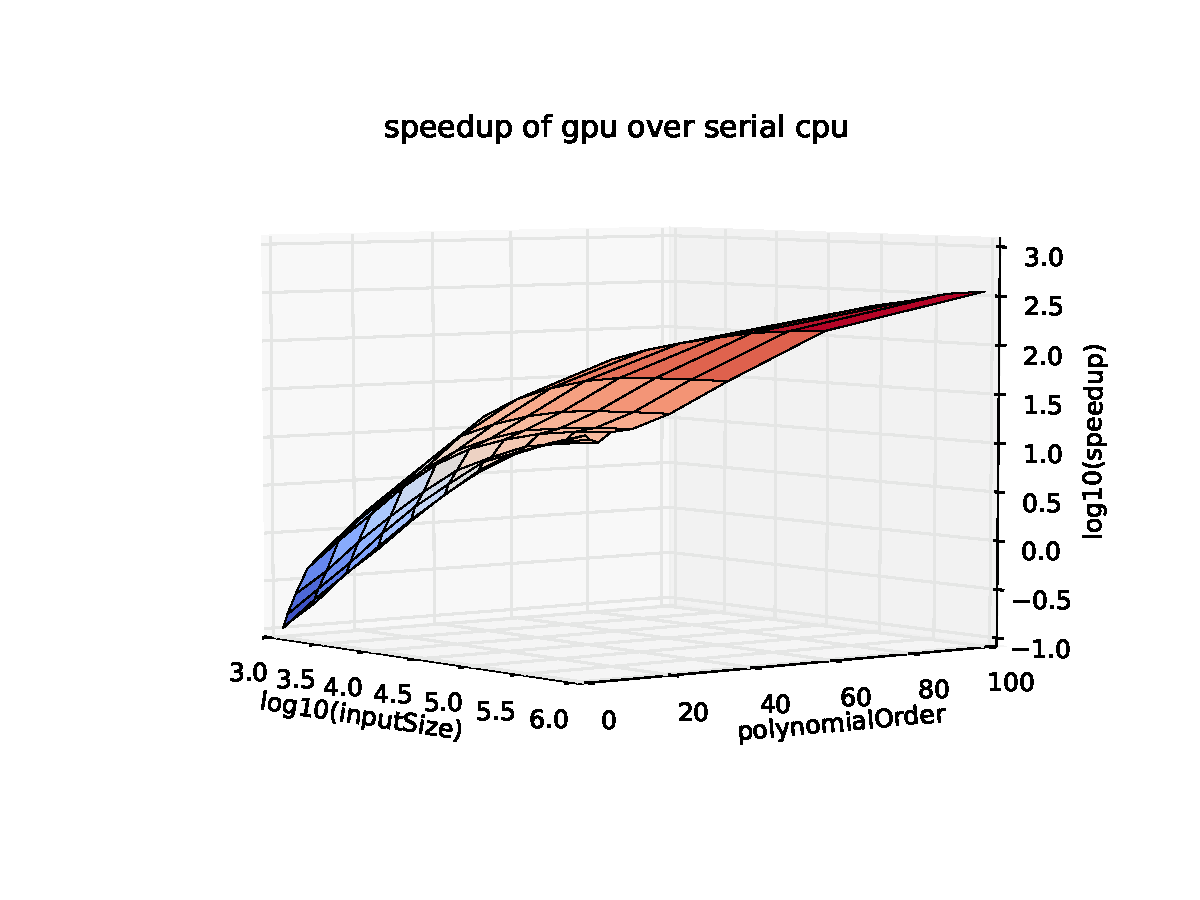
\includegraphics[width=4.40in, trim=.75in .5in .50in 0in, clip]{figures/Main4_versusInputSizeAndOrder_shuffler}} \\
    \subfloat[versus blocks and threads for a large input size and large polynomial order]{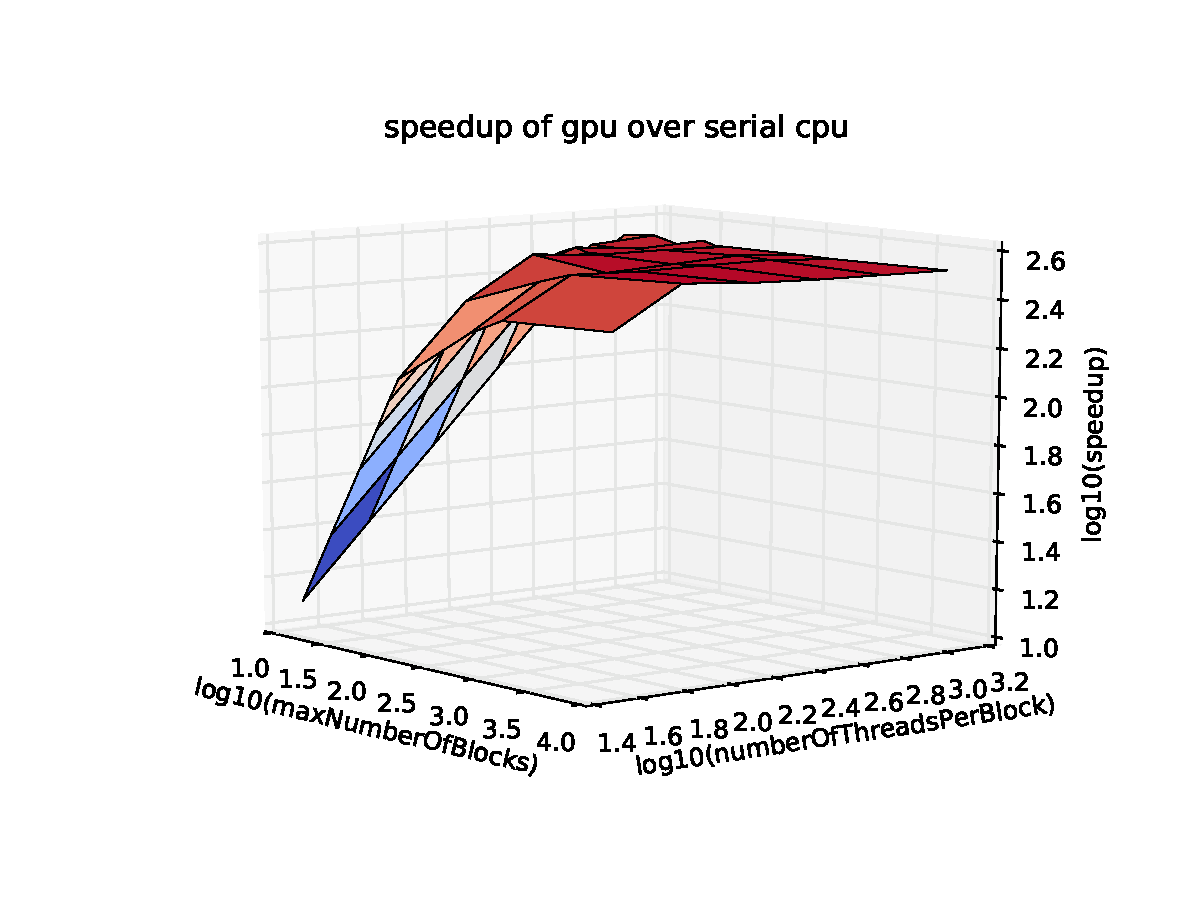
\includegraphics[width=4.40in, trim=.75in .5in .50in 0in, clip]{figures/Main4_versusBlocksAndThreads_shuffler}} \\
    \end{tabular}
    \end{center}
    \caption{Performance of cuda polynomials}
    \label{fig:Main4}
  \end{figure}
}

\fi

\FloatBarrier

\vfill







\eprob{15}{Back to the Real World}

Provide short (but sufficient) answers to the following prompts:

\begin{enumerate}[a)]
\item Explain as you would to a ``non-technical'' friend of yours what hyperthreading is.

\ifSolutions
\textbf{Solution:}

\fi

\item Explain as you would to a ``non-technical'' friend of yours what ``context switching'' is.

\ifSolutions
\textbf{Solution:}

\fi

\item Explain as you would to a ``non-technical'' friend of yours what ``cache cooling'' is.

\ifSolutions
\textbf{Solution:}

\fi

\item Explain as you would to a ``non-technical'' friend of yours what ``cache thrashing'' is.

\ifSolutions
\textbf{Solution:}

\fi

\end{enumerate}

\vfill

\eprob{5}{Feedback}

\begin{enumerate}[a)]
\item How much total time did you spend on this assignment?
\item Of the total time, how much total time did you spend ``flailing'' on little annoying things that are not the main point of the assignment?
\item Of the total time, how much total time did you spend on stretch problems?
\item Did you have any ``aha'' moments where something clicked?  If so, on what problems or parts?
\item Can you give me any feedback on this assignment?
\end{enumerate}

\vfill

\vskip 1cm
\total


\end{document}

todo: find a way to make stretch problems worth more than the rest of the assignment

